\documentclass[a4paper,12pt]{article}
\usepackage[utf8]{inputenc}
\usepackage[T1]{fontenc}
\usepackage{graphicx}
\usepackage{hyperref}
\usepackage{listings}
\usepackage{amsmath}
\usepackage{float}
\usepackage{geometry}
\usepackage{polski}
\usepackage{color}

\geometry{margin=1in}

\title{Sprawozdanie z laboratorium 2}
\author{Mikołaj Kubś 272662}
\date{\today}

\begin{document}

\maketitle

\section{Cel zadania}
Celem zadania było zapoznanie się z procesem tworzenia prostych stron Single Page Application (SPA), a także integracją z Azure Static Web i Github Pages. Dodatkowo wykorzystano technikę leniwego ładowania i mechanizm reCAPTCHA.

\subsection{Wprowadzenie}
Single Page Application (SPA) to rodzaj aplikacji internetowej, w której nawigacja odbywa się poprzez asynchroniczne ładowanie poszczególnych elementów strony, takich jak sekcje lub całe widoki, bez konieczności przeładowywania całej strony. Dzięki temu użytkownik doświadcza płynniejszej interakcji, ponieważ zmiany w interfejsie są natychmiastowe i nie wymagają pełnego odświeżenia przeglądarki.

W aplikacjach SPA cała zawartość jest zazwyczaj ładowana jednorazowo przy pierwszym wejściu na stronę, a późniejsze interakcje z użytkownikiem prowadzą do dynamicznej aktualizacji wyświetlanych danych za pomocą JavaScript. To podejście pozwala na szybsze działanie aplikacji oraz lepsze wykorzystanie zasobów sieciowych, ponieważ jedynie zmieniane elementy są przesyłane między serwerem a klientem.

\subsection{Tworzenie aplikacji SPA z wykorzystaniem HTML i JS}

\subsubsection{Kod HTML}
Plik \texttt{index.html} definiuje prosty kod HTML aplikacji:

\begin{figure}[H]
    \centering
    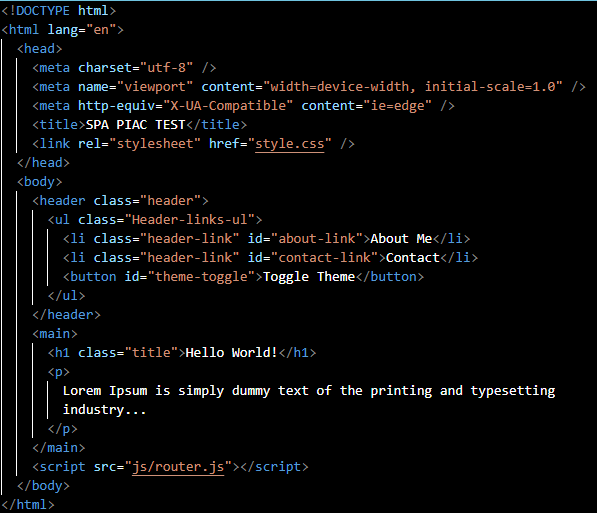
\includegraphics[width=1\textwidth]{images/index_html.png}
    \caption{Kod index.html}
\end{figure}

Kod wewnątrz <main> jest podmieniany przez \texttt{router.js}.

\subsubsection{Stylizacja CSS}
Plik \texttt{style.css} definiuje kaskadowe arkusze stylów:

\begin{figure}[H]
    \centering
    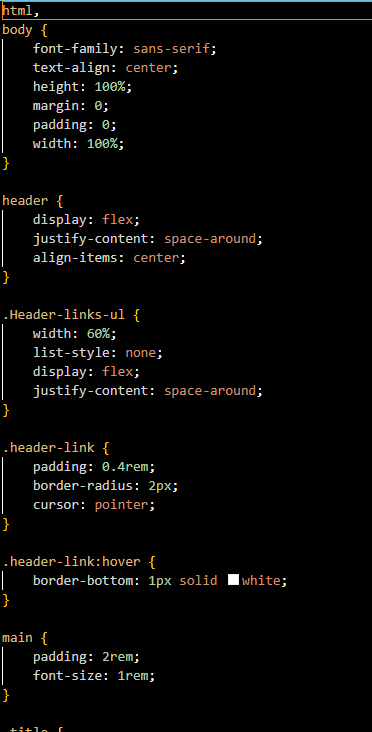
\includegraphics[width=1\textwidth]{images/css.png}
    \caption{Fragment kodu style.css}
\end{figure}

\subsubsection{Kod JavaScript}
Plik \texttt{router.js} zarządza nawigacją w aplikacji SPA:

\begin{figure}[H]
    \centering
    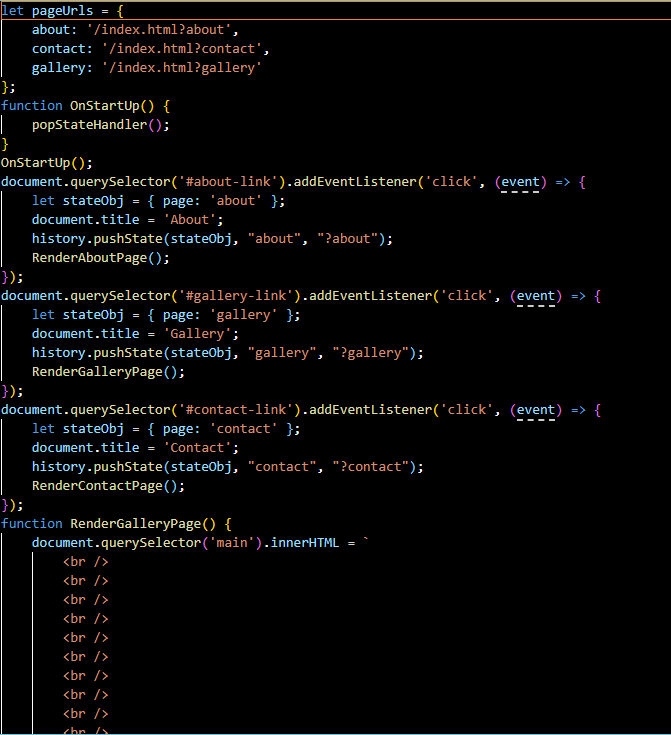
\includegraphics[width=1\textwidth]{images/js.png}
    \caption{Fragment kodu router.js}
\end{figure}

\subsubsection{Leniwe ładowanie}

Do implementacji leniwego ładowania obrazków wykorzystano Intersection Observer API. Obrazki są tworzone dynamicznie, a atrybut \texttt{src} jest przypisany dopiero, gdy obrazki powinny być widoczne. Obrazki są ładowane jako Blob.

\begin{figure}[H]
    \centering
    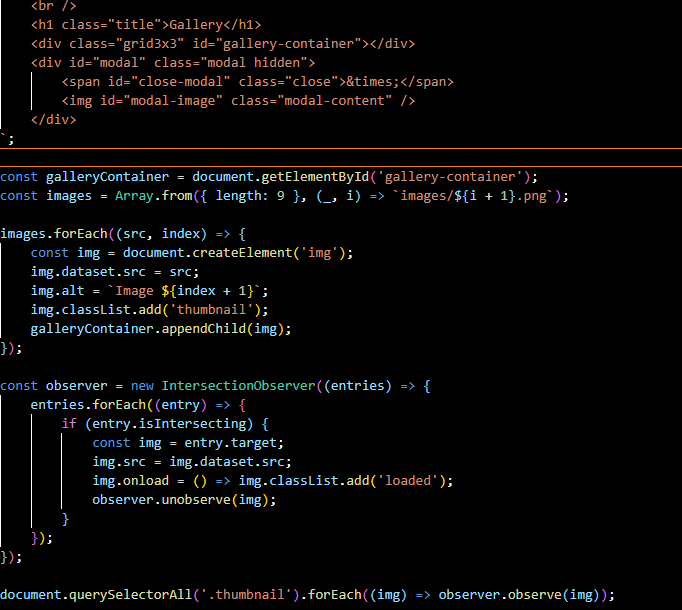
\includegraphics[width=1\textwidth]{images/lazy.png}
    \caption{Fragment kodu odpowiedzialnego za leniwe ładowanie}
\end{figure}

\begin{figure}[H]
    \centering
    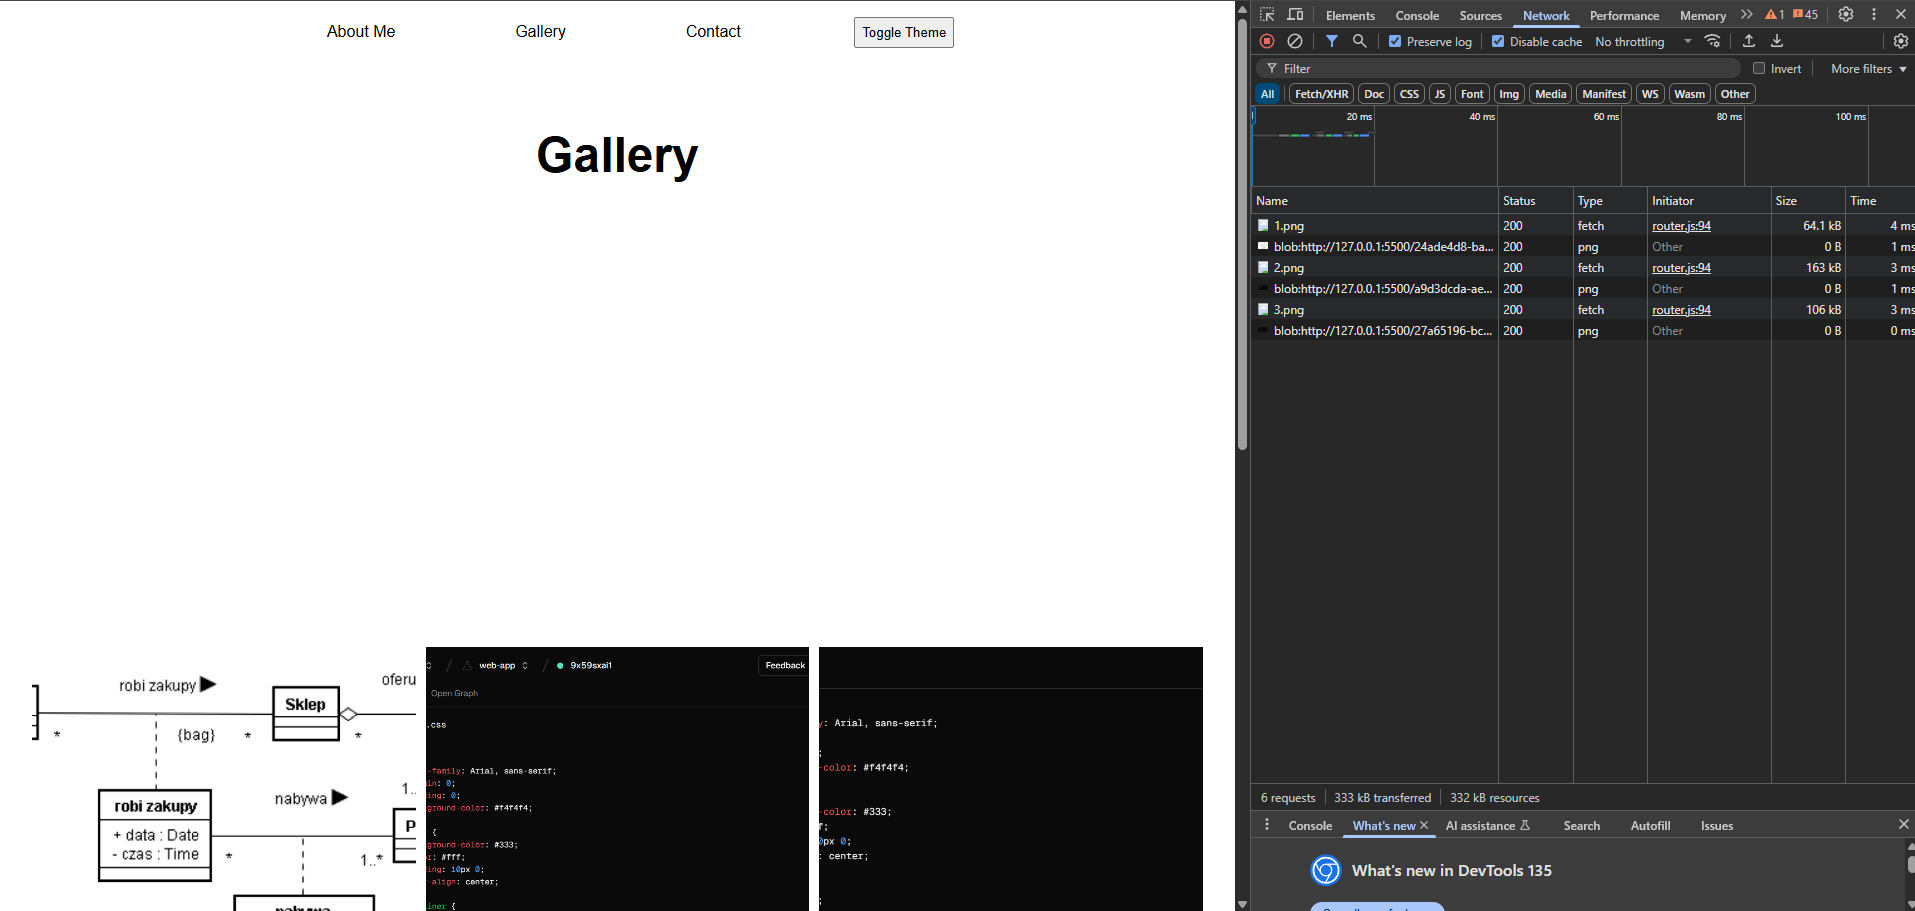
\includegraphics[width=1\textwidth]{images/gallery.png}
    \caption{Galeria w aplikacji}
\end{figure}

\begin{figure}[H]
    \centering
    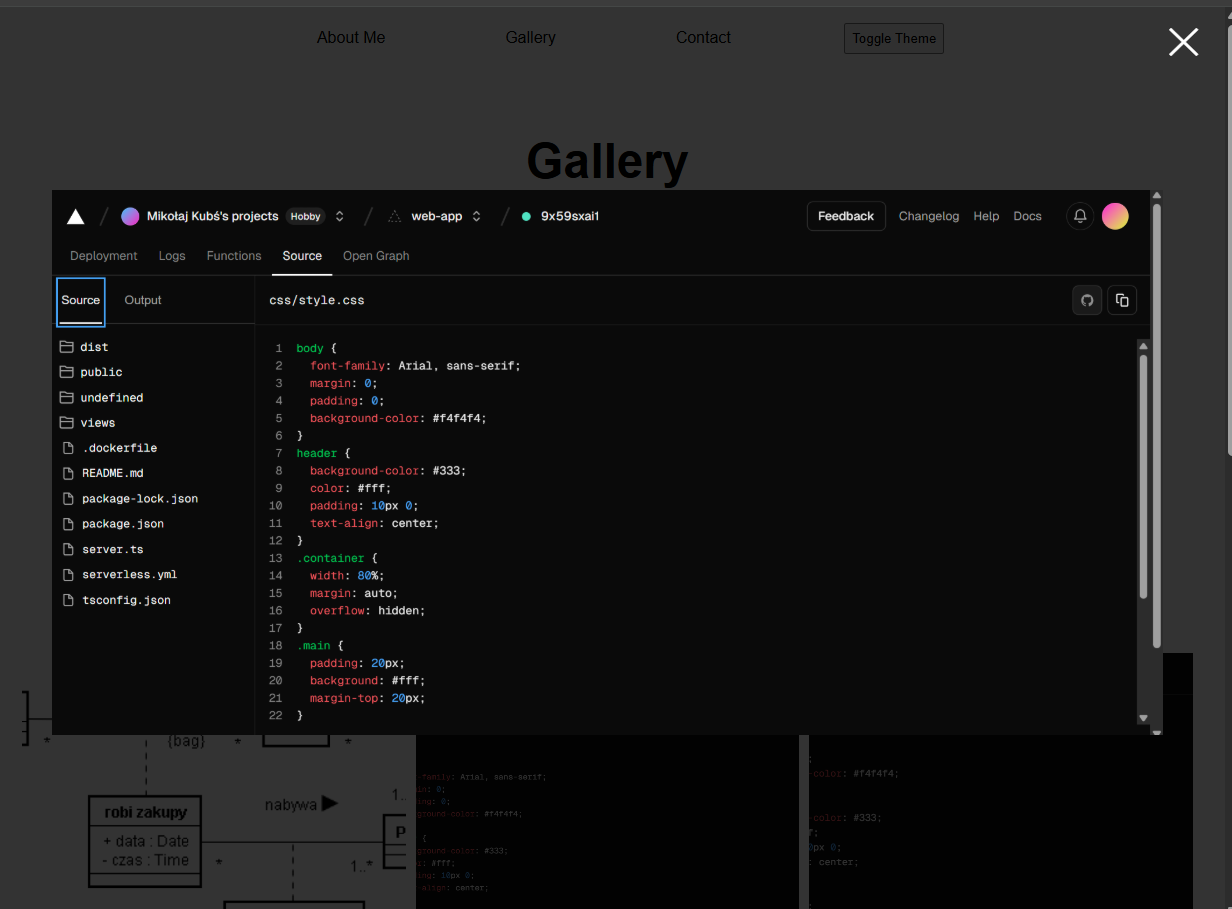
\includegraphics[width=1\textwidth]{images/modal.png}
    \caption{Modalne okno obrazka}
\end{figure}

\subsubsection{Implementacja reCAPTCHA}

Należało przypisać domenę w systemie reCAPTCHA Google. Grecaptcha renderuje widget Google, a w form jej wysłanie jest przechwycone i sprawdzone, czy grecaptcha nie zwraca błędu.

\begin{figure}[H]
    \centering
    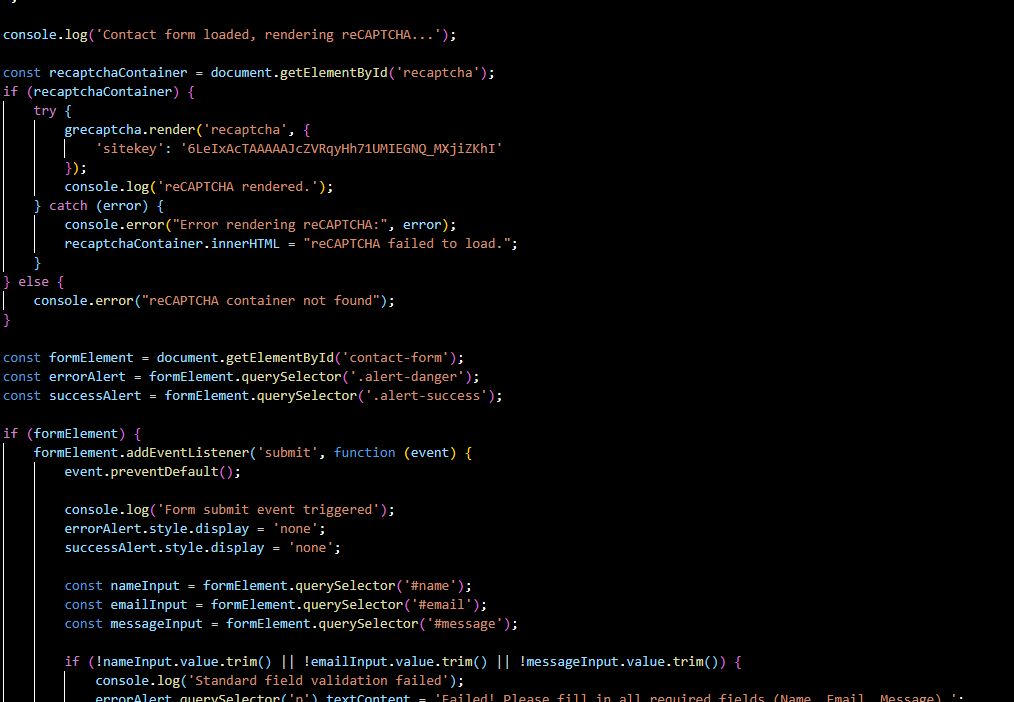
\includegraphics[width=1\textwidth]{images/recaptcha.png}
    \caption{Fragment kodu odpowiedzialnego za mechanizm reCAPTCHA}
\end{figure}

\begin{figure}[H]
    \centering
    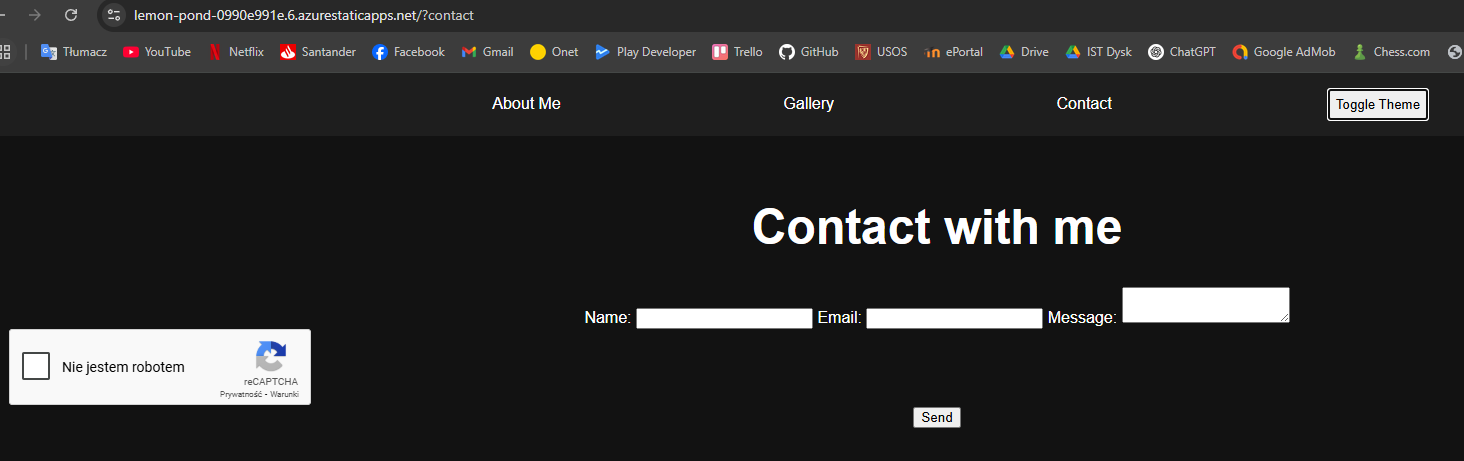
\includegraphics[width=1\textwidth]{images/contact.png}
    \caption{Strona kontakt w aplikacji}
\end{figure}

\subsection{Wdrożenie aplikacji w środowisku chmurowym}
\subsubsection{Azure Static Web Apps}
Azure Static Web Apps oferuje darmową usługę hostingową dla aplikacji SPA. Kroki wdrożenia:
\begin{enumerate}
    \item Zaloguj się na \url{https://portal.azure.com}.
    \item Utwórz nową aplikację statyczną, podając szczegóły projektu.
    \item Połącz aplikację z repozytorium GitHub.
    \item Wdróż aplikację i sprawdź jej działanie.
\end{enumerate}

Wdrożenie aplikacji zadziałało bezproblemowo. Po zcommitowaniu kodu na GitHub i poczekaniu, aż Azure to przetworzy, zmieni się hostowana wersja aplikacji.

\subsubsection{GitHub Pages}
GitHub Pages umożliwia hostowanie aplikacji SPA. Kroki wdrożenia:
\begin{enumerate}
    \item Utwórz repozytorium na GitHubie.
    \item Skonfiguruj GitHub Pages w ustawieniach repozytorium.
    \item Sprawdź dostępność aplikacji pod adresem \texttt{https://username.github.io/repository}.
\end{enumerate}

Różne pliki były hostowane na \texttt{https://github.com/lmProgramming/lmProgramming.github.io} od dawna - głównie informacji dla botów reklamowych Google'a oraz polityki prywatności gier autora. Dodanie nowej struktury strony przebiegło bezproblemowo.

\begin{figure}[H]
    \centering
    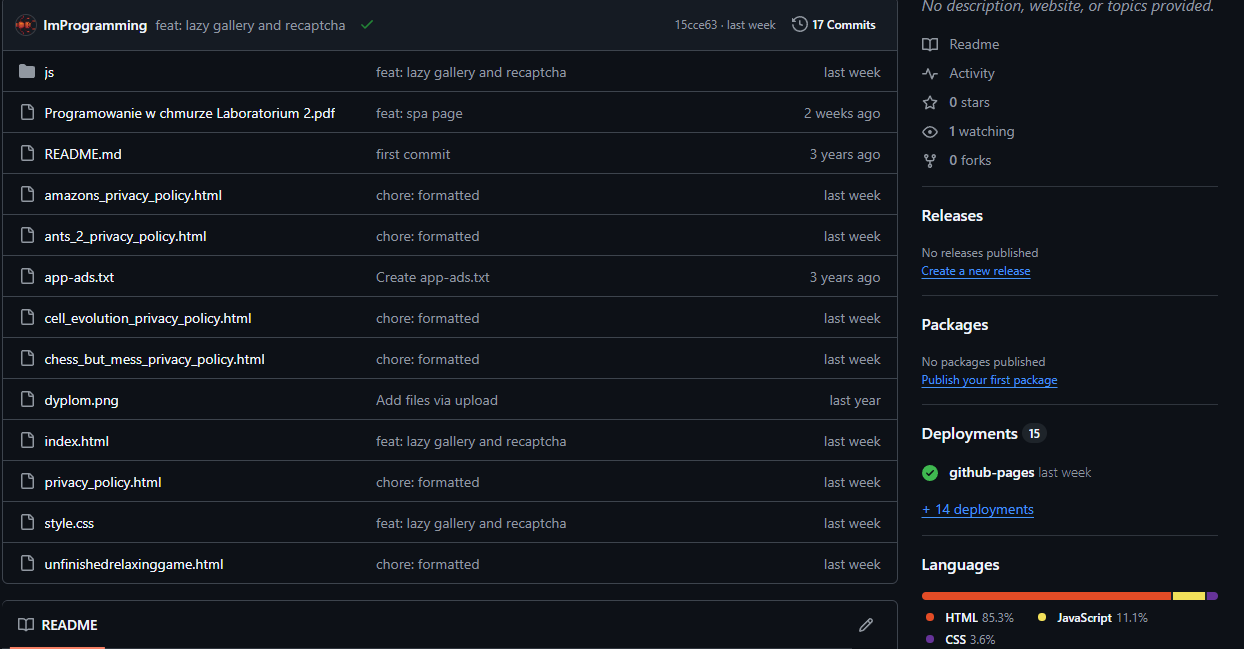
\includegraphics[width=1\textwidth]{images/github.png}
    \caption{Udany deployment na Github pages.}
\end{figure}

\subsection{Testowanie aplikacji}
Przeprowadzone testy aplikacji:
\begin{itemize}
    \item Sprawdź nawigację między stronami.
    \item Zweryfikuj poprawność ładowania obrazów w galerii.
    \item Przetestuj walidację formularza kontaktowego.
    \item Użyj narzędzia Lighthouse w ChromeDevTools do analizy wydajności.
\end{itemize}

\subsubsection{Nawigacja}

Nawigacja działa bezproblemowo, wszystkie stany są zapisane w historii. Nawigacja jest praktycznie natychmiastowa.

\subsubsection{Leniwe ładowanie}

\begin{figure}[H]
    \centering
    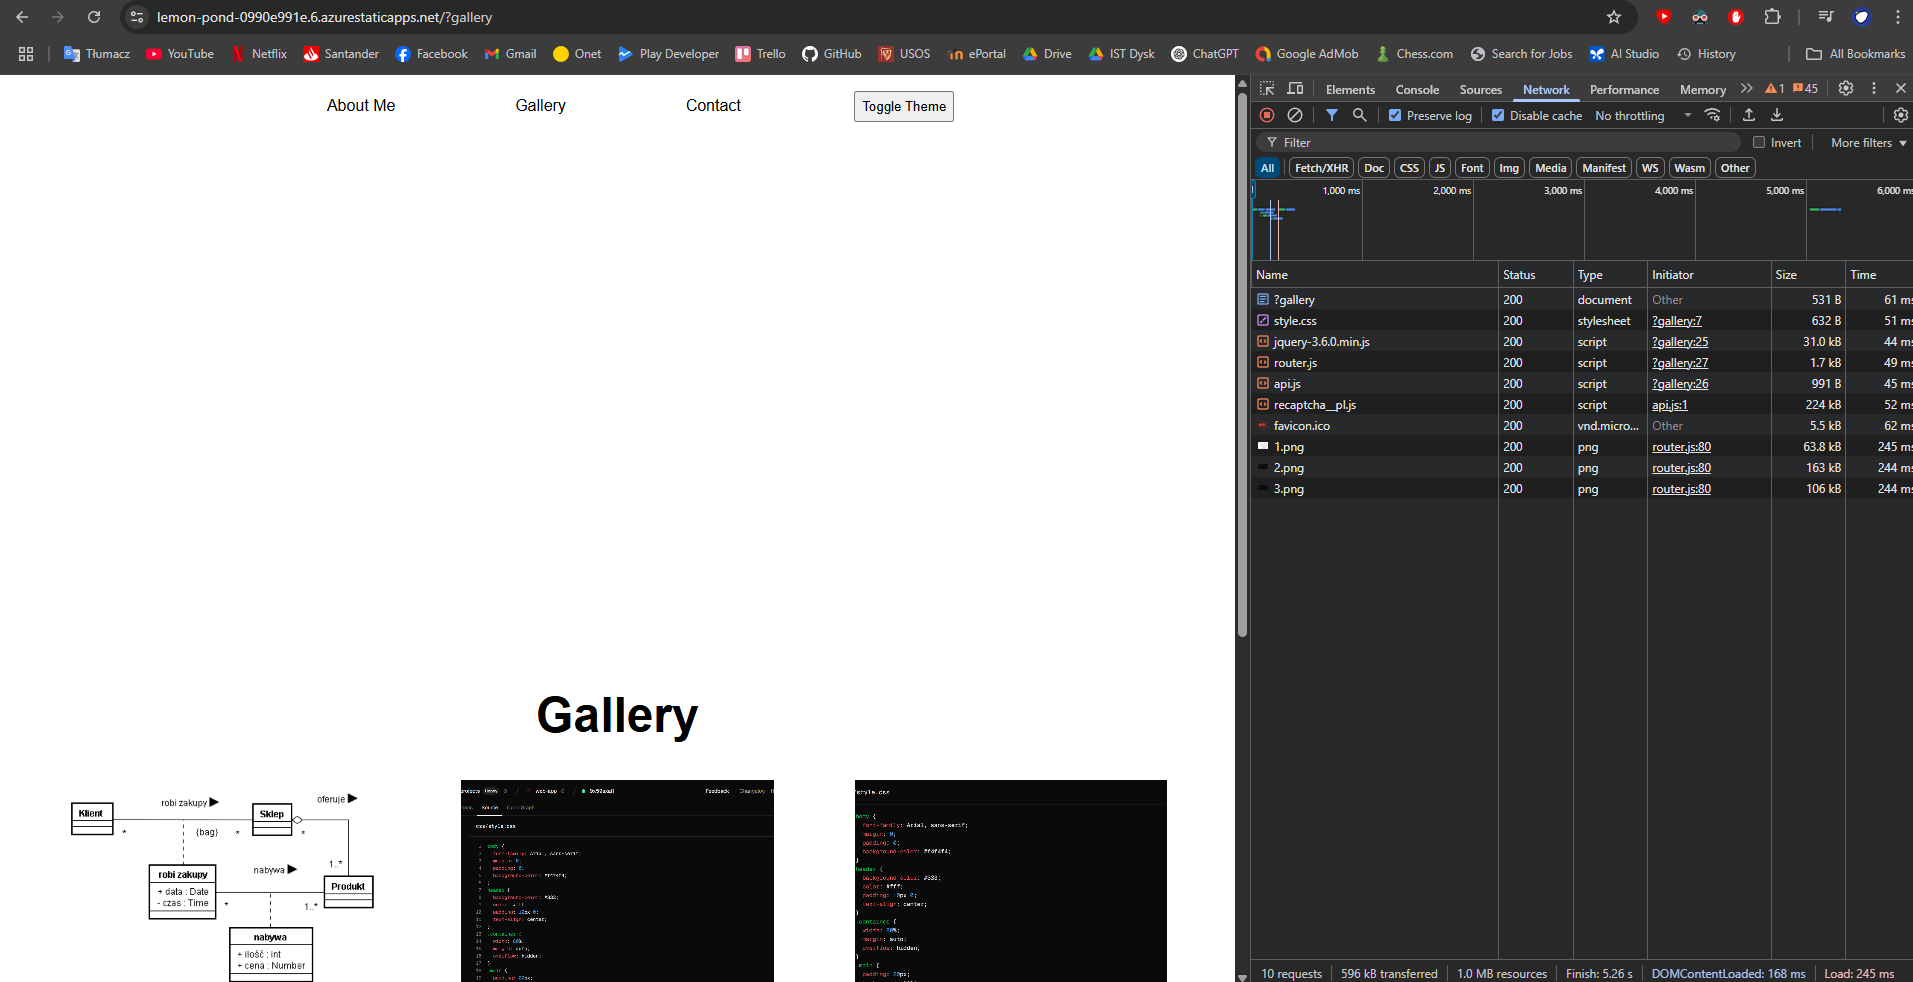
\includegraphics[width=1\textwidth]{images/lazy_2.png}
    \caption{Tylko 3 z 9 obrazków załadowana, co oznacza, że leniwe ładowanie działa.}
\end{figure}

\subsubsection{ReCAPTCHA}

\begin{figure}[H]
    \centering
    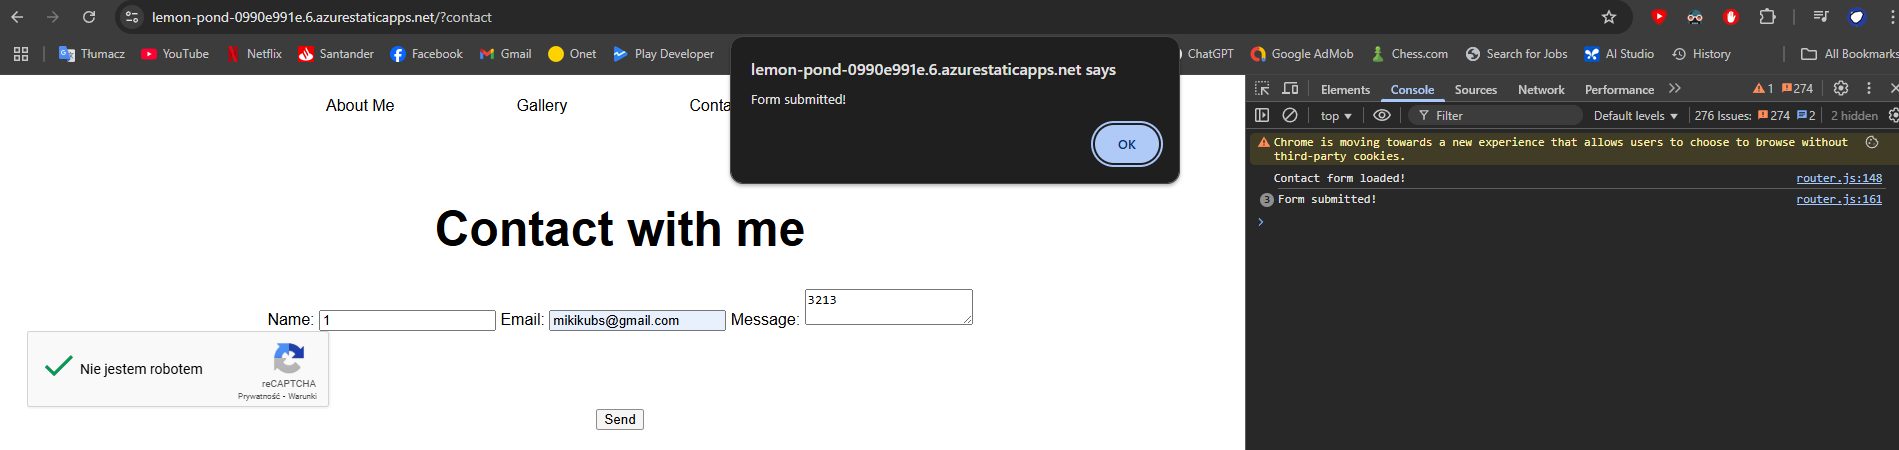
\includegraphics[width=1\textwidth]{images/contact_success.png}
    \caption{Sukces wysłania formularza z reCAPTCHA.}
\end{figure}

Przez test aplikacji na innej domenie, mechanizm reCAPTCHA nie może działać - wysłanie formularza nie uda się.

\begin{figure}[H]
    \centering
    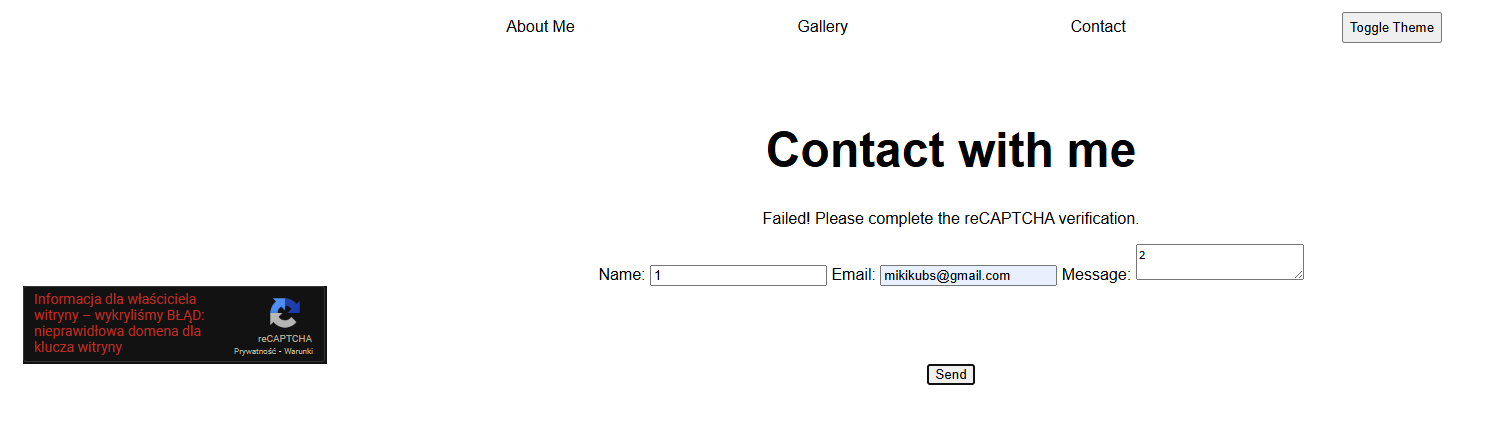
\includegraphics[width=1\textwidth]{images/contact_failure.png}
    \caption{Nieudane wysłanie formularza z reCAPTCHA.}
\end{figure}

\subsubsection{Lighthouse}

Lighthouse pomaga mierzyć i diagnozować problemy z wydajnością ładowania, interaktywnością (TBT), dostępnością (ważne dla wszystkich użytkowników), SEO (kluczowe dla SPA) i ogólnymi dobrymi praktykami webowymi.

\begin{figure}[H]
    \centering
    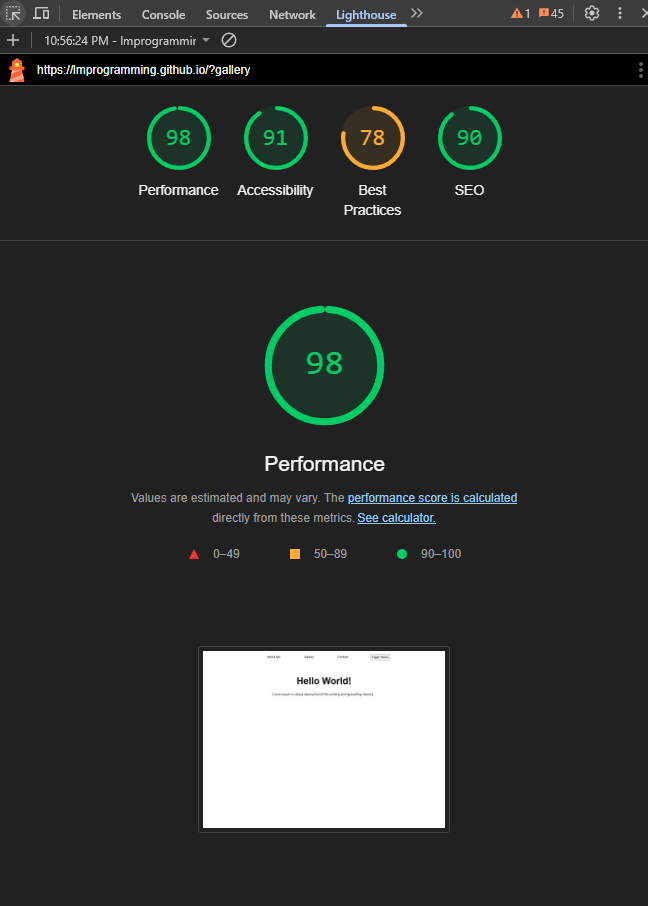
\includegraphics[width=1\textwidth]{images/lighthouse.png}
    \caption{Wynik analizy Lighthouse.}
\end{figure}

Wynik analizy performance to aż 98/100, co oznacza wynik bardzo dobry, nie ma potrzeby go polepszać.

\begin{figure}[H]
    \centering
    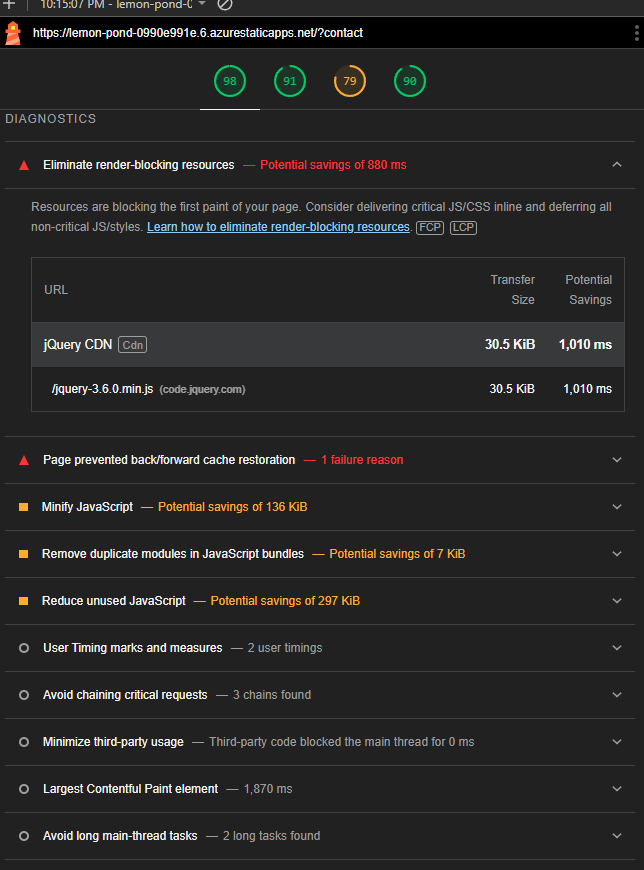
\includegraphics[width=1\textwidth]{images/lighthouse_details.png}
    \caption{Szczegóły analizy Lighthouse.}
\end{figure}

\subsubsection{Inna przeglądarka i rozdzielczość}

\begin{figure}[H]
    \centering
    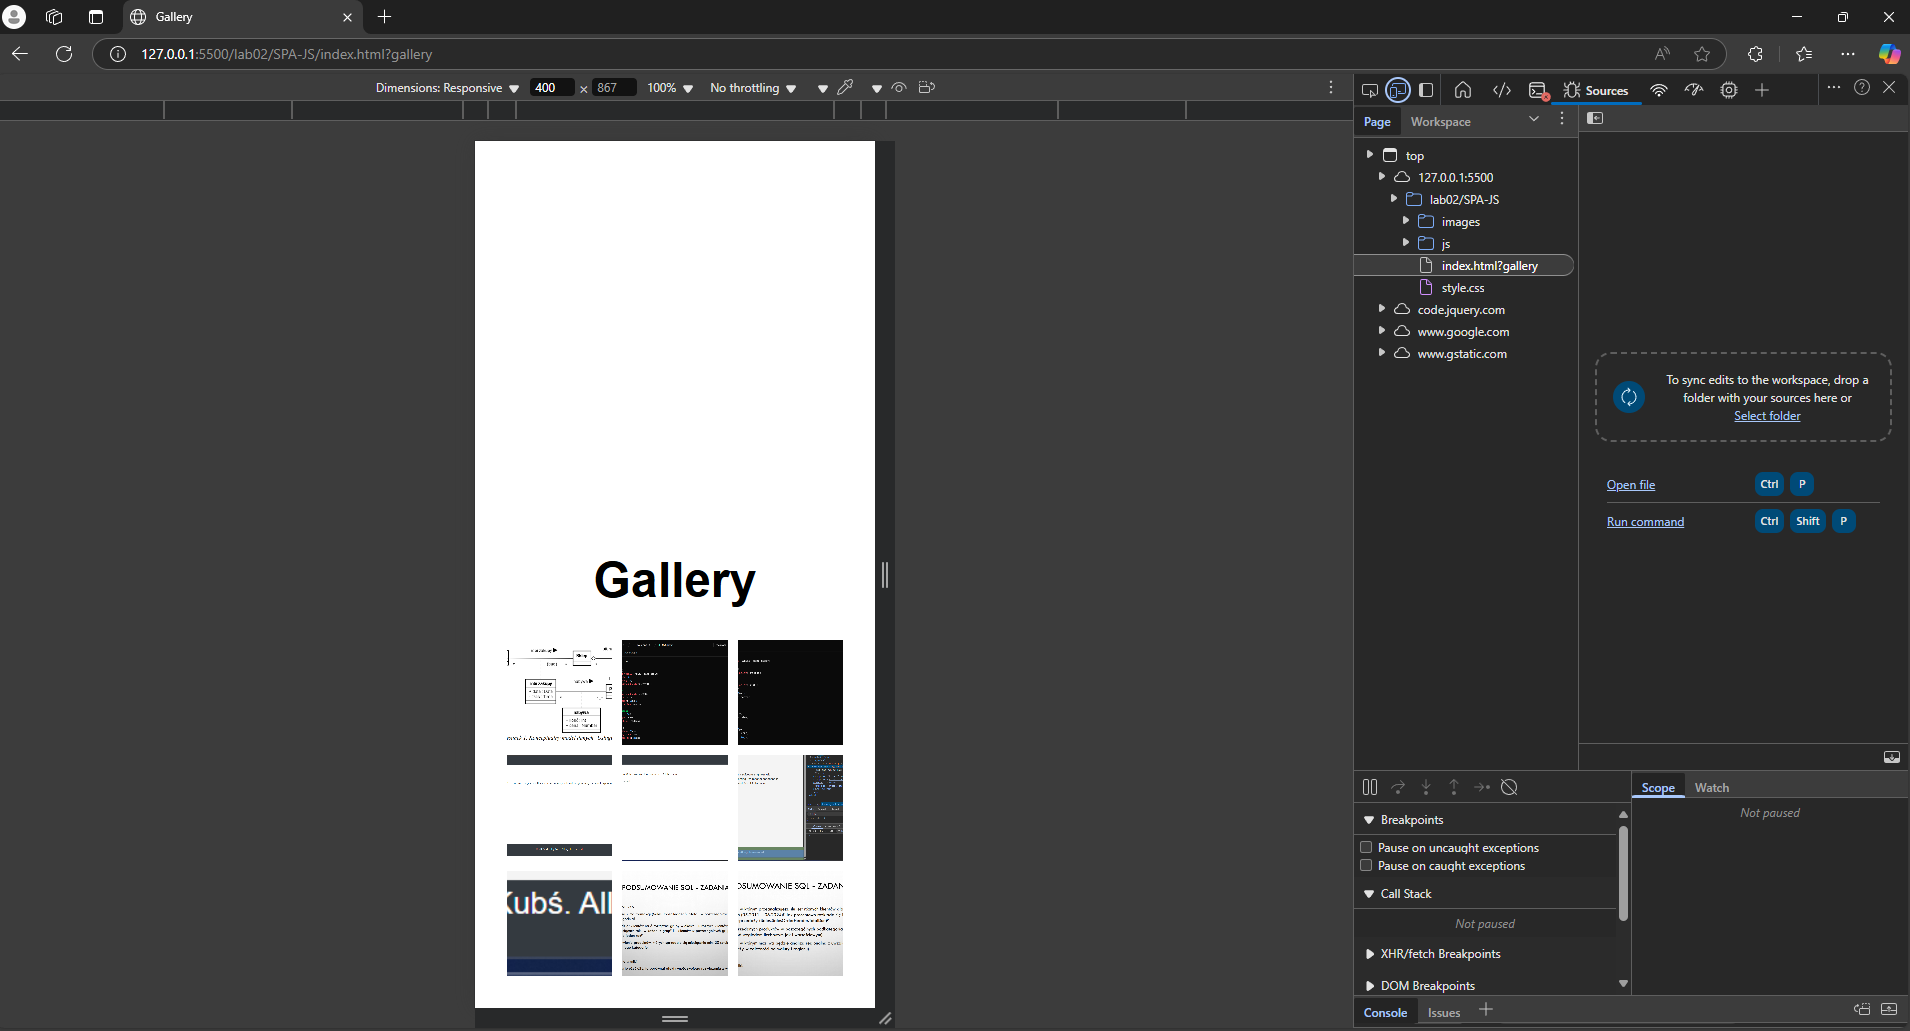
\includegraphics[width=1\textwidth]{images/edge.png}
    \caption{Poprawne wyświetlanie strony w przeglądarce Edge, symulując wymiary telefonu}
\end{figure}

\section{Wyzwania związane z SPA}

\begin{itemize}
    \item Routing po stronie klienta
    \item Problemy z zarządzaniem stanu aplikacji
    \item Optymalizacja pierwszego załadowania strony (skoro wymaga pobrania większej liczby stron na początku)
    \item Zwłaszcza kiedyś występowały problemy z SEO i SPA, teraz ten problem jest mniejszy dzięki lepszym robotom Google
    \item Bezpieczeństwo - większa ilość logiki po stronie klienta otwiera nowe możliwości ataku
\end{itemize}

\end{document}
